\documentclass[report.tex]{subfiles}
\graphicspath{ \subfix{./images/} \subfix{./graphs/} }
\begin{document}
\section{Milestone 3: Implement the Judger}

\subsection{Implementation and testing}

The Judger needs to be initialized with a working directory path for it to store all the temporary files. A folder path and the file name of the source code is taken as arguments.

\begin{minted}{csharp}
/// <summary>
/// Set the SourceCode File with its folder path and its name.
/// </summary>
/// <param name="FolderPath"></param>
/// <param name="FileName"></param>
public static void SetSourceCodeFilePath(string FolderPath, string FileName = "main")
{
    _SourceCodeFolderPath = FolderPath;
    _SourceCodeFilePath = Path.Combine(FolderPath, FileName) + "{SourceCodeFileExtension}";
    _ExecutableFilePath = Path.Combine(FolderPath, FileName) + ".exe";
}
\end{minted}

Next, I started implementing the \code{Compile} function. It is a static function, so it can be called without creating an instance of the class. It is also an async function, so when it is executing, it will not block the main UI thread. This is particularly important as the user interface should stay responsive when the judger is working. It returns a \code{Task<int>} value, which contains the exit code of the compiler.

To allow the user to customize the behaviour of different compilers, the compile command supports magic variables SourceCodeFileExtension, SourceCodeFilePath and ExecutableFilePath. These variables need to be replaced with the real value before executing.

\begin{minted}{csharp}
/// <summary>
/// Compile the source code in <see cref="_SourceCodeFilePath"/>.
/// </summary>
/// <param name="language">
/// The <see cref="Language.CompileCommand"/> and 
/// <see cref="Language.CompileArguments"/> are used for compilation.
/// Note that the <see cref="Language.NeedCompile"/> is not checked.
/// </param>
/// <returns>The exit code of the compiler is returned.</returns>
private async static Task<int> Compile(Language language)
{
    // Clear old output
    _CompilationOutput = "";
    _CompilationError = "";

    // Set file extension
    string sourceFilePath = _SourceCodeFilePath.Replace("{SourceCodeFileExtension}", language.FileExtension);

    // Create compile process
    Process CompileProcess = new()
    {
        StartInfo = new ProcessStartInfo
        {
            FileName = language.CompileCommand
                .Replace("{SourceCodeFilePath}", sourceFilePath)
                .Replace("{ExecutableFilePath}", _ExecutableFilePath),
            Arguments = language.CompileArguments
                .Replace("{SourceCodeFilePath}", sourceFilePath)
                .Replace("{ExecutableFilePath}", _ExecutableFilePath),
            UseShellExecute = false,
            CreateNoWindow = true,
            RedirectStandardOutput = true,
            RedirectStandardError = true,
            WorkingDirectory = _SourceCodeFolderPath
        },
        EnableRaisingEvents = true
    };

    // Bind event handler
    CompileProcess.OutputDataReceived +=
        new DataReceivedEventHandler(CompileProcess_OutputDataReceived);
    CompileProcess.ErrorDataReceived +=
        new DataReceivedEventHandler(CompileProcess_ErrorDataReceived);

    // Start the process
    CompileProcess.Start();
    CompileProcess.BeginOutputReadLine();
    CompileProcess.BeginErrorReadLine();

    // Wait for exit
    await CompileProcess.WaitForExitAsync();
    return CompileProcess.ExitCode;
}
\end{minted}

Two event handlers are bound to the \code{CompileProcess}. They are simply used to receive the output from the compiler. They are bost set to private to encapsulate from the main program.

\begin{minted}{csharp}
private static void CompileProcess_ErrorDataReceived(object sender, DataReceivedEventArgs e)
{
    if (!string.IsNullOrEmpty(e.Data))
    {
        _CompilationError += e.Data + '\n';
    }
}

private static void CompileProcess_OutputDataReceived(object sender, DataReceivedEventArgs e)
{
    if (!string.IsNullOrEmpty(e.Data))
    {
        _CompilationOutput += e.Data + '\n';
    }
}
\end{minted}

The \code{Execute} procedure follows the same pattern.

\begin{minted}{csharp}
/// <summary>
/// Execute the executable in <see cref="_ExecutableFilePath"/>.
/// </summary>
/// <param name="stdin">The standard input gets feeded to the program.</param>
/// <param name="language">The language config contains the running config.</param>
/// <param name="timeLimit">The time limit for the process.</param>
/// <param name="memoryLimit">The memory limit for the process.</param>
/// <returns></returns>
private async static Task<int> Execute(string stdin, Language language, int timeLimit, long memoryLimit)
{
    // Clear the old data
    _StandardOutput = "";
    _StandardError = "";
    _StatusCode = StatusCode.PENDING;
    _WorkingSet64 = 0;

    // Set file extension
    string sourceFilePath = _SourceCodeFilePath.Replace("{SourceCodeFileExtension}", language.FileExtension);

    // Create the execute process
    Process ExecuteProcess = new()
    {
        StartInfo = new ProcessStartInfo
        {
            FileName = language.RunCommand
                .Replace("{SourceCodeFilePath}", sourceFilePath)
                .Replace("{ExecutableFilePath}", _ExecutableFilePath),
            Arguments = language.RunArguments
                .Replace("{SourceCodeFilePath}", sourceFilePath)
                .Replace("{ExecutableFilePath}", _ExecutableFilePath),
            UseShellExecute = false,
            RedirectStandardInput = true,
            RedirectStandardOutput = true,
            RedirectStandardError = true,
            CreateNoWindow = true,
            WorkingDirectory = _SourceCodeFolderPath
        },
        EnableRaisingEvents = true
    };

    // Bind the event handler
    ExecuteProcess.OutputDataReceived +=
        new DataReceivedEventHandler(ExecuteProcess_OutputDataReceived);
    ExecuteProcess.ErrorDataReceived +=
        new DataReceivedEventHandler(ExecuteProcess_ErrorDataReceived);
    ExecuteProcess.Exited +=
        new EventHandler(ExecuteProcess_Exited);

    // Start running
    ExecuteProcess.Start();
    ExecuteProcess.BeginOutputReadLine();
    ExecuteProcess.BeginErrorReadLine();
    ExecuteProcess.StandardInput.WriteLine(stdin);
    _StatusCode = StatusCode.RUNNING;

    // Wait for exit
    await ExecuteProcess.WaitForExitAsync();
    return ExecuteProcess.ExitCode;
}
\end{minted}

On top of the running procedure, I also need to monitor the memory and time usage and kill the process when the limit is exceeded.

\begin{minted}{csharp}
// Start the time monitor
Timer timer = new((e) =>
{
    if (_StatusCode == StatusCode.RUNNING && ExecuteProcess.HasExited == false)
    {
        ExecuteProcess.Kill();
        _StatusCode = StatusCode.TIME_LIMIT_EXCEEDED;
    }
}, null, timeLimit, Timeout.Infinite);
\end{minted}

This is a count down timer, it runs on a separate thread, once the time limit is reached, it executes the kill command and records the TLE.

\begin{minted}{csharp}
// Create the memory monitor
Thread MemoryMonitor = new(() =>
{
    while (ExecuteProcess.HasExited == false)
    {
        ExecuteProcess.Refresh();
        _WorkingSet64 = ExecuteProcess.PeakWorkingSet64;
        if (_WorkingSet64 > memoryLimit)
        {
            ExecuteProcess.Kill();
            _StatusCode = StatusCode.MEMORY_LIMIT_EXCEEDED;
        }
    }
});
\end{minted}

This is a memory monitor, it runs on a separate thread too. It keeps refreshing the process information and checking the memory usage. If the memory usage exceeds the limit, it kills the process and records the MLE error.

I use a \code{RunCode} function to combime these two steps together, and returns a \code{RunCodeResult} containing all data.

\begin{minted}{csharp}
/// <summary>
/// Run the UserCode with the given data.
/// Use the Progress for reporting progress.
/// </summary>
/// <param name="UserCode"></param>
/// <param name="Input"></param>
/// <param name="language"></param>
/// <param name="TimeLimit"></param>
/// <param name="MemoryLimit"></param>
/// <param name="Progress"></param>
/// <returns></returns>
public async static Task<RunCodeResult> RunCode(string UserCode, string Input, Language language, int TimeLimit, long MemoryLimit, IProgress<int> Progress)
{
    Progress.Report(0);

    // Set file extension
    string sourceFilePath = _SourceCodeFilePath.Replace("{SourceCodeFileExtension}", language.FileExtension);

    // Save the code to the disk
    RunCodeResult result = new();
    Directory.CreateDirectory(_SourceCodeFolderPath);
    await File.WriteAllTextAsync(sourceFilePath, UserCode);

    // Compile if needed
    if (language.NeedCompile)
    {
        // Compile and report any error
        if (await Compile(language) != 0)
        {
            Progress.Report(100);
            result.StandardOutput = _CompilationOutput;
            result.StandardError = FilterErrorMessage(_CompilationError);
            result.ResultCode = ResultCode.COMPILE_ERROR;
            return result;
        }
    }
    // Finish compilation
    Progress.Report(10);

    // Setup watch
    var watch = new Stopwatch();
    watch.Start();

    // Execute the code
    result.ExitCode = await Execute(Input, language, TimeLimit, MemoryLimit);
    
    // Save the results
    watch.Stop();
    result.StandardOutput = _StandardOutput;
    result.StandardError = FilterErrorMessage(_StandardError);
    result.CPUTime = watch.ElapsedMilliseconds;
    result.MemoryUsage = _WorkingSet64;

    // Report complete
    Progress.Report(100);

    return result;
}
\end{minted}

Before the result is returned, its status needs to be determined. I use a series of branching to convert the internal state to a final status code.

\begin{minted}{csharp}
// Handle TLE
if (_StatusCode == StatusCode.TIME_LIMIT_EXCEEDED)
{
    result.ResultCode = ResultCode.TIME_LIMIT_EXCEEDED;
    return result;
}

// Handle MLE
if (_StatusCode == StatusCode.MEMORY_LIMIT_EXCEEDED)
{
    result.ResultCode = ResultCode.MEMORY_LIMIT_EXCEEDED;
    return result;
}

// Handle RE
if (!string.IsNullOrEmpty(result.StandardError) || result.ExitCode != 0)
{
    result.ResultCode = ResultCode.RUNTIME_ERROR;
    return result;
}

// Success
result.ResultCode = ResultCode.SUCCESS;
\end{minted}

To test the basic functionality, I set up two test cases. The code simply outputs hello world and the Judger asserts whether the output is correct. I choose to test on two different programming languages, Python and C++ since Python is an interpreting language and C++ is a compiled language, which tests the Judger's full functionality.

\begin{minted}{csharp}
[TestClass]
public class TestJudger
{
    const int MB = 1024 * 1024;
    const int S = 1000;
    const string helloWorldPy = "print('hello world')";
    const string helloWorldCpp = "#include <iostream>\nusing namespace std;\nint main(){cout << \"hello world\" << endl;}";
    
    [TestInitialize]
    public void SetCodeFilePath()
    {
        Judger.SetSourceCodeFilePath(".", "main");
    }

    /// <summary>
    /// Test running a simple hello world Python program
    /// </summary>
    /// <returns></returns>
    [TestMethod, TestCategory("TestRunCode")]
    public async Task TestRunCodePython()
    {
        RunCodeResult result = await Judger.RunCode(helloWorldPy, "", LanguageConfig.Python, 1 * S, 64 * MB);
        Assert.AreEqual("hello world\n", result.StandardOutput);
        Assert.AreEqual("", result.StandardError);
        Assert.AreEqual(0, result.ExitCode);
        Assert.IsTrue(result.CPUTime < 2 * ms && result.CPUTime > 0);
        Assert.IsTrue(result.MemoryUsage < 128 * MB && result.MemoryUsage > 0);
        Assert.AreEqual(ResultCode.SUCCESS, result.ResultCode);
    }

    /// <summary>
    /// Test running a simple hello world C++ program
    /// </summary>
    /// <returns></returns>
    [TestMethod, TestCategory("TestRunCode")]
    public async Task TestRunCodeCpp()
    {
        RunCodeResult result = await Judger.RunCode(helloWorldCpp, "", LanguageConfig.Cpp, 1 * S, 64 * MB);
        Assert.AreEqual("hello world\n", result.StandardOutput);
        Assert.AreEqual("", result.StandardError);
        Assert.AreEqual(0, result.ExitCode);
        Assert.IsTrue(result.CPUTime < 2 * ms && result.CPUTime > 0);
        Assert.IsTrue(result.MemoryUsage < 128 * MB && result.MemoryUsage > 0);
        Assert.AreEqual(ResultCode.SUCCESS, result.ResultCode);
    }
}
\end{minted}

These tests passed without an issue.

\begin{minted}{text}
> dotnet test --filter TestCategory=TestRunCode
  Determining projects to restore...
  All projects are up-to-date for restore.
  Algorithm Dynamics.Core -> C:\Algorithm-Dynamics\src\Algorithm Dynamics.Core\bin\Debug\net6.0\Algorithm Dynamics.Core.dll
  Algorithm Dynamics.Test -> C:\Algorithm-Dynamics\src\Algorithm Dynamics.Test\bin\Debug\net6.0\Algorithm Dynamics.Test.dll
Test run for C:\Algorithm-Dynamics\src\Algorithm Dynamics.Test\bin\Debug\net6.0\Algorithm Dynamics.Test.dll (.NETCoreApp,Version=v6.0)
Microsoft (R) Test Execution Command Line Tool Version 17.0.0
Copyright (c) Microsoft Corporation.  All rights reserved.

Starting test execution, please wait...
A total of 1 test files matched the specified pattern.

Passed!  - Failed:     0, Passed:     2, Skipped:     0, Total:     2, Duration: 651 ms - Algorithm Dynamics.Test.dll (net6.0)
\end{minted}

Next, I tested input. I use the simple A + B problem, two integers will be fed to the test code by the judger, and a correct sum should be output.

\begin{minted}{csharp}
const string APlusBPy = "a=int(input())\nb=int(input())\nprint(a+b)";
const string APlusBCpp = "#include <iostream>\nusing namespace std;\nint main(){int a,b;cin>>a>>b;cout<<a+b;}";

/// <summary>
/// Test input processing
/// </summary>
/// <returns></returns>
[TestMethod, TestCategory("TestRunCodeInput")]
public async Task TestRunCodeInputPy()
{
    RunCodeResult result = await Judger.RunCode(APlusBPy, "3\n4", LanguageConfig.Python, 1 * S, 64 * MB);
    Assert.AreEqual("7\n", result.StandardOutput);
    Assert.AreEqual("", result.StandardError);
    Assert.AreEqual(0, result.ExitCode);
    Assert.IsTrue(result.CPUTime < 2 * ms && result.CPUTime > 0);
    Assert.IsTrue(result.MemoryUsage < 128 * MB && result.MemoryUsage > 0);
    Assert.AreEqual(ResultCode.SUCCESS, result.ResultCode);
}

/// <summary>
/// Test input processing
/// </summary>
/// <returns></returns>
[TestMethod, TestCategory("TestRunCodeInput")]
public async Task TestRunCodeInputCpp()
{
    RunCodeResult result = await Judger.RunCode(APlusBCpp, "3\n4", LanguageConfig.Cpp, 1 * S, 64 * MB);
    Assert.AreEqual("7\n", result.StandardOutput);
    Assert.AreEqual("", result.StandardError);
    Assert.AreEqual(0, result.ExitCode);
    Assert.IsTrue(result.CPUTime < 2 * ms && result.CPUTime > 0);
    Assert.IsTrue(result.MemoryUsage < 128 * MB && result.MemoryUsage > 0);
    Assert.AreEqual(ResultCode.SUCCESS, result.ResultCode);
}
\end{minted}

Both tests passed successfully.

\begin{minted}{text}
> dotnet test --filter TestCategory=TestRunCodeInput
  Determining projects to restore...
  All projects are up-to-date for restore.
  Algorithm Dynamics.Core -> C:\Algorithm-Dynamics\src\Algorithm Dynamics.Core\bin\Debug\net6.0\Algorithm Dynamics.Core.dll
  Algorithm Dynamics.Test -> C:\Algorithm-Dynamics\src\Algorithm Dynamics.Test\bin\Debug\net6.0\Algorithm Dynamics.Test.dll
Test run for C:\Algorithm-Dynamics\src\Algorithm Dynamics.Test\bin\Debug\net6.0\Algorithm Dynamics.Test.dll (.NETCoreApp,Version=v6.0)
Microsoft (R) Test Execution Command Line Tool Version 17.0.0
Copyright (c) Microsoft Corporation.  All rights reserved.

Starting test execution, please wait...
A total of 1 test files matched the specified pattern.

Passed!  - Failed:     0, Passed:     2, Skipped:     0, Total:     2, Duration: 796 ms - Algorithm Dynamics.Test.dll (net6.0)
\end{minted}

Next, I test the time limit. I input a piece of code that will run an infinite loop. The Judger is expected to kill the process after 1 second and report the correct error.

\begin{minted}{csharp}
const string TLEPy = "while True:\n    pass";
const string TLECpp = "int main(){while(1){}}";

/// <summary>
/// Test time limit exceed
/// </summary>
/// <returns></returns>
[TestMethod, TestCategory("TestTLE")]
public async Task TestTLEPy()
{
    RunCodeResult result = await Judger.RunCode(TLEPy, "", LanguageConfig.Python, 1 * S, 64 * MB);
    Assert.AreEqual("", result.StandardOutput);
    Assert.AreEqual("", result.StandardError);
    Assert.AreNotEqual(0, result.ExitCode);
    Assert.IsTrue(result.CPUTime >= 1 * S);
    Assert.IsTrue(result.MemoryUsage < 128 * MB && result.MemoryUsage > 0);
    Assert.AreEqual(ResultCode.TIME_LIMIT_EXCEEDED, result.ResultCode);
}

/// <summary>
/// Test time limit exceed
/// </summary>
/// <returns></returns>
[TestMethod, TestCategory("TestTLE")]
public async Task TestTLECpp()
{
    RunCodeResult result = await Judger.RunCode(TLECpp, "", LanguageConfig.Cpp, 1 * S, 64 * MB);
    Assert.AreEqual("", result.StandardOutput);
    Assert.AreEqual("", result.StandardError);
    Assert.AreNotEqual(0, result.ExitCode);
    Assert.IsTrue(result.CPUTime >= 1 * S);
    Assert.IsTrue(result.MemoryUsage < 128 * MB && result.MemoryUsage > 0);
    Assert.AreEqual(ResultCode.TIME_LIMIT_EXCEEDED, result.ResultCode);
}
\end{minted}

Both tests passed successfully.

\begin{minted}{text}
> dotnet test --filter TestCategory=TestTLE
  Determining projects to restore...
  All projects are up-to-date for restore.
  Algorithm Dynamics.Core -> C:\Algorithm-Dynamics\src\Algorithm Dynamics.Core\bin\Debug\net6.0\Algorithm Dynamics.Core.dll
  Algorithm Dynamics.Test -> C:\Algorithm-Dynamics\src\Algorithm Dynamics.Test\bin\Debug\net6.0\Algorithm Dynamics.Test.dll
Test run for C:\Algorithm-Dynamics\src\Algorithm Dynamics.Test\bin\Debug\net6.0\Algorithm Dynamics.Test.dll (.NETCoreApp,Version=v6.0)
Microsoft (R) Test Execution Command Line Tool Version 17.0.0
Copyright (c) Microsoft Corporation.  All rights reserved.

Starting test execution, please wait...
A total of 1 test files matched the specified pattern.

Passed!  - Failed:     0, Passed:     2, Skipped:     0, Total:     2, Duration: 2 s - Algorithm Dynamics.Test.dll (net6.0)
\end{minted}

Next, I test the memory limit. I input a piece of code that will use a large amount of memory. The Judger is expected to kill the process when the actual memory usage is more than 64 MB.

\begin{minted}{csharp}
const string MLEPy = "a=[1]\nwhile True:\n    a+=a";
const string MLECpp = "const int N = 100000000;int a[N];int main(){for(int i = 0;i<N;i++)a[i]= i;}";

/// <summary>
/// Test memory limit exceed
/// </summary>
/// <returns></returns>
[TestMethod, TestCategory("TestMLE")]
public async Task TestMLEPy()
{
    RunCodeResult result = await Judger.RunCode(MLEPy, "", LanguageConfig.Python, 1 * S, 64 * MB);
    Assert.AreEqual("", result.StandardOutput);
    Assert.AreEqual("", result.StandardError);
    Assert.AreNotEqual(0, result.ExitCode);
    Assert.IsTrue(result.CPUTime < 2 * ms && result.CPUTime > 0);
    Assert.IsTrue(result.MemoryUsage > 64 * MB);
    Assert.AreEqual(ResultCode.MEMORY_LIMIT_EXCEEDED, result.ResultCode);
}

/// <summary>
/// Test memory limit exceed
/// </summary>
/// <returns></returns>
[TestMethod, TestCategory("TestMLE")]
public async Task TestMLECpp()
{
    RunCodeResult result = await Judger.RunCode(MLECpp, "", LanguageConfig.Cpp, 1 * S, 64 * MB, null, true);
    Assert.AreEqual("", result.StandardOutput);
    Assert.AreEqual("", result.StandardError);
    Assert.AreNotEqual(0, result.ExitCode);
    Assert.IsTrue(result.CPUTime < 2 * ms && result.CPUTime > 0);
    Assert.IsTrue(result.MemoryUsage > 64 * MB);
    Assert.AreEqual(ResultCode.MEMORY_LIMIT_EXCEEDED, result.ResultCode);
}
\end{minted}

Next, I test the compile error. I input a piece of code that will not compile. The Judger is expected to collect the error message from the compiler and report it in the result.

\begin{minted}{csharp}
const string CECpp = "ce";

/// <summary>
/// Test compile error
/// </summary>
/// <returns></returns>
[TestMethod, TestCategory("TestCE")]
public async Task TestCE()
{
    RunCodeResult result = await Judger.RunCode(CECpp, "", LanguageConfig.Cpp, 1 * S, 64 * MB);
    Assert.AreEqual("", result.StandardOutput);
    Assert.AreNotEqual("", result.StandardError);
    Assert.AreEqual(0, result.ExitCode);
    Assert.AreEqual(0, result.CPUTime);
    Assert.AreEqual(0, result.MemoryUsage);
    Assert.AreEqual(ResultCode.COMPILE_ERROR, result.ResultCode);
}
\end{minted}

The test passes successfully.

\begin{minted}{text}
> dotnet test --filter TestCategory=TestCE
  Determining projects to restore...
  All projects are up-to-date for restore.
  Algorithm Dynamics.Core -> C:\Algorithm-Dynamics\src\Algorithm Dynamics.Core\bin\Debug\net6.0\Algorithm Dynamics.Core.dll
  Algorithm Dynamics.Test -> C:\Algorithm-Dynamics\src\Algorithm Dynamics.Test\bin\Debug\net6.0\Algorithm Dynamics.Test.dll
Test run for C:\Algorithm-Dynamics\src\Algorithm Dynamics.Test\bin\Debug\net6.0\Algorithm Dynamics.Test.dll (.NETCoreApp,Version=v6.0)
Microsoft (R) Test Execution Command Line Tool Version 17.0.0
Copyright (c) Microsoft Corporation.  All rights reserved.

Starting test execution, please wait...
A total of 1 test files matched the specified pattern.

Passed!  - Failed:     0, Passed:     1, Skipped:     0, Total:     1, Duration: 104 ms - Algorithm Dynamics.Test.dll (net6.0)
\end{minted}

Next, I test the runtime error. For interpreting language like Python, the syntax is checked during runtime. The Judger is expected to collect the error message from the interpreter and report it in the result.

\begin{minted}{csharp}
const string REPy = "re";

/// <summary>
/// Test runtime error
/// </summary>
/// <returns></returns>
[TestMethod, TestCategory("TestRE")]
public async Task TestRE()
{
    RunCodeResult result = await Judger.RunCode(REPy, "", LanguageConfig.Python, 1 * S, 64 * MB);
    Assert.AreEqual("", result.StandardOutput);
    Assert.AreNotEqual("", result.StandardError);
    Assert.AreNotEqual(0, result.ExitCode);
    Assert.IsTrue(result.CPUTime > 0 && result.CPUTime < 2 * S);
    Assert.IsTrue(result.MemoryUsage > 0 && result.MemoryUsage < 64 * MB);
    Assert.AreEqual(ResultCode.RUNTIME_ERROR, result.ResultCode);
}
\end{minted}

The test passed successfully.

\begin{minted}{text}
> dotnet test --filter TestCategory=TestRE
  Determining projects to restore...
  All projects are up-to-date for restore.
  Algorithm Dynamics.Core -> C:\Algorithm-Dynamics\src\Algorithm Dynamics.Core\bin\Debug\net6.0\Algorithm Dynamics.Core.dll
  Algorithm Dynamics.Test -> C:\Algorithm-Dynamics\src\Algorithm Dynamics.Test\bin\Debug\net6.0\Algorithm Dynamics.Test.dll
Test run for C:\Algorithm-Dynamics\src\Algorithm Dynamics.Test\bin\Debug\net6.0\Algorithm Dynamics.Test.dll (.NETCoreApp,Version=v6.0)
Microsoft (R) Test Execution Command Line Tool Version 17.0.0
Copyright (c) Microsoft Corporation.  All rights reserved.

Starting test execution, please wait...
A total of 1 test files matched the specified pattern.

Passed!  - Failed:     0, Passed:     1, Skipped:     0, Total:     1, Duration: 100 ms - Algorithm Dynamics.Test.dll (net6.0)
\end{minted}

I then implement the judge test case and judge problem function. This is a pretty straightforward task because I can reuse the entire \code{RunCode} function. On top of the result given by the \code{RunCode} function, I add a branch to determine whether the result is correct and report a wrong answer when the output does not match.

\begin{minted}{csharp}
/// <summary>
/// Judge a TestCase
/// </summary>
/// <param name="UserCode"></param>
/// <param name="TestCase"></param>
/// <param name="Language"></param>
/// <param name="TimeLimit"></param>
/// <param name="MemoryLimit"></param>
/// <returns></returns>
public async static Task<TestCaseResult> JudgeTestCase(string UserCode, TestCase TestCase, Language Language, int TimeLimit, long MemoryLimit)
{
    RunCodeResult runCodeResult = await RunCode(UserCode, TestCase.Input, Language, TimeLimit, MemoryLimit, new Progress<int>());
    
    // Handle WA
    if (runCodeResult.ResultCode == ResultCode.SUCCESS)
    {
        if (runCodeResult.StandardOutput.Trim() != TestCase.Output.Trim())
        {
            runCodeResult.ResultCode = ResultCode.WRONG_ANSWER;
        }
    }

    // Not implemented edit result so must create it at the end
    TestCaseResult result = TestCaseResult.Create(runCodeResult);
    return result;
}
\end{minted}

I set up 2 sets of tests to test the \code{JudgeTestCase} function. The first one test it with a simple hello world code to make sure it is working as intended. The second test is with a wrong answer code, to see whether it reports the correct error.

\begin{minted}{csharp}
/// <summary>
/// Test judge <see cref="TestCase"/>
/// </summary>
/// <returns></returns>
[TestMethod, TestCategory("TestTestCase")]
public async Task TestTestCaseCpp()
{
    DataAccess.InitializeDatabase($"{Guid.NewGuid()}.db");
    TestCase testCase = TestCase.Create("", "hello world\n", false);
    TestCaseResult result = await Judger.JudgeTestCase(helloWorldCpp, testCase, LanguageConfig.Cpp, 1 * S, 64 * MB);
    Assert.AreEqual("hello world\n", result.StandardOutput);
    Assert.AreEqual("", result.StandardError);
    Assert.AreEqual(0, result.ExitCode);
    Assert.IsTrue(result.CPUTime < 2 * S && result.CPUTime > 0);
    Assert.IsTrue(result.MemoryUsage < 128 * MB && result.MemoryUsage > 0);
    Assert.AreEqual(ResultCode.SUCCESS, result.ResultCode);
}

/// <summary>
/// Test Wrong Answer
/// </summary>
/// <returns></returns>
[TestMethod, TestCategory("TestWrongAnswer")]
public async Task TestWrongAnswerPy()
{
    DataAccess.InitializeDatabase($"{Guid.NewGuid()}.db");
    TestCase testCase = TestCase.Create("3\n4\n", "7", false);
    TestCaseResult result = await Judger.JudgeTestCase(WAPy, testCase, LanguageConfig.Python, 1 * S, 64 * MB);
    Assert.AreEqual(0, result.ExitCode);
    Assert.IsTrue(result.CPUTime > 0 && result.CPUTime < 2 * S);
    Assert.IsTrue(result.MemoryUsage > 0 && result.MemoryUsage < 128 * MB);
    Assert.AreEqual(ResultCode.WRONG_ANSWER, result.ResultCode);
    Assert.AreNotEqual("7", result.StandardOutput);
    Assert.AreEqual("", result.StandardError);
}

/// <summary>
/// Test Wrong Answer
/// </summary>
/// <returns></returns>
[TestMethod, TestCategory("TestWrongAnswer")]
public async Task TestWrongAnswerCpp()
{
    DataAccess.InitializeDatabase($"{Guid.NewGuid()}.db");
    TestCase testCase = TestCase.Create("3\n4\n", "7", false);
    TestCaseResult result = await Judger.JudgeTestCase(WACpp, testCase, LanguageConfig.Cpp, 1 * S, 64 * MB);
    Assert.AreEqual(0, result.ExitCode);
    Assert.IsTrue(result.CPUTime > 0 && result.CPUTime < 2 * S);
    Assert.IsTrue(result.MemoryUsage > 0 && result.MemoryUsage < 128 * MB);
    Assert.AreEqual(ResultCode.WRONG_ANSWER, result.ResultCode);
    Assert.AreNotEqual("7", result.StandardOutput);
    Assert.AreEqual("", result.StandardError);
}
\end{minted}

All tests passed successfully.

\begin{minted}{text}
> dotnet test --filter TestCategory="TestWrongAnswer|TestTestCase"
  Determining projects to restore...
  All projects are up-to-date for restore.
  Algorithm Dynamics.Core -> C:\Algorithm-Dynamics\src\Algorithm Dynamics.Core\bin\Debug\net6.0\Algorithm Dynamics.Core.dll
  Algorithm Dynamics.Test -> C:\Algorithm-Dynamics\src\Algorithm Dynamics.Test\bin\Debug\net6.0\Algorithm Dynamics.Test.dll
Test run for C:\Algorithm-Dynamics\src\Algorithm Dynamics.Test\bin\Debug\net6.0\Algorithm Dynamics.Test.dll (.NETCoreApp,Version=v6.0)
Microsoft (R) Test Execution Command Line Tool Version 17.0.0
Copyright (c) Microsoft Corporation.  All rights reserved.

Starting test execution, please wait...
A total of 1 test files matched the specified pattern.

Passed!  - Failed:     0, Passed:     4, Skipped:     0, Total:     4, Duration: 2 s - Algorithm Dynamics.Test.dll (net6.0)
\end{minted}

To judge a problem, I set up a queue of test cases, judge them one by one, and compose the result at the end.

\begin{minted}{csharp}
/// <summary>
/// Judge a problem submission
/// </summary>
/// <param name="Submission"></param>
/// <param name="Progress"></param>
/// <returns></returns>
public async static Task<SubmissionResult> JudgeProblem(Submission Submission, IProgress<int> Progress)
{
    // Create SubmissionResult
    SubmissionResult Result = SubmissionResult.Create(Submission, new());

    // Set up Judge Queue
    Queue<TestCase> JudgeQueue = new(Submission.Problem.TestCases);

    // Ready to judge, report progress
    Progress.Report(0);

    int testCasesCount = Submission.Problem.TestCases.Count;
    while (JudgeQueue.Count > 0)
    {
        TestCaseResult result = await JudgeTestCase(
            Submission.Code,
            JudgeQueue.Dequeue(),
            Submission.Language,
            Submission.Problem.TimeLimit,
            Submission.Problem.MemoryLimit);

        // Add result
        Result.AddTestCaseResult(result);

        // Report progress
        Progress.Report(100 * (testCasesCount - JudgeQueue.Count) / testCasesCount);
    }

    //Finish Judging
    Progress.Report(100);

    // Update problem status
    if (Result.ResultCode == ResultCode.SUCCESS)
    {
        Submission.Problem.Status = ProblemStatus.Solved;
    }
    else
    {
        if (Submission.Problem.Status == ProblemStatus.Todo)
        {
            Submission.Problem.Status = ProblemStatus.Attempted;
        }
    }

    return Result;
}
\end{minted}

I add a set of simple tests just to see \code{JudgeProblem} is working correctly. I generate 100 test cases for the A + B problem and test it on both Python and C++.

\begin{minted}{csharp}
/// <summary>
/// Test Judge Problem
/// </summary>
/// <returns></returns>
[TestMethod, TestCategory("TestJudgeProblem")]
public async Task TestJudgeProblemPy()
{
    DataAccess.InitializeDatabase($"{Guid.NewGuid()}.db");

    // Generate 1000 A + B test cases
    Random rnd = new();
    List<TestCase> testCases = new();
    for (int i = 0; i < 100; i ++)
    {
        int a = rnd.Next(1000);
        int b = rnd.Next(1000);
        testCases.Add(TestCase.Create($"{a}\n{b}\n", $"{a + b}\n", false));
    }
    
    // Generate problem
    Problem problem = Problem.Create(Guid.NewGuid(), "", "", 1 * S, 64 * MB, Difficulty.Easy, testCases);

    // Generate submission
    User user = DatabaseHelper.CreateNewUser();
    Language language = DatabaseHelper.CreateLanguage("python");
    Submission submission = Submission.Create(APlusBPy, language, user, problem);
    SubmissionResult result = await Judger.JudgeProblem(submission, new Progress<int>());

    // Run tests
    Assert.AreEqual("Success", result.Result);
    Assert.AreEqual(ResultCode.SUCCESS, result.ResultCode);
    Assert.IsTrue(0 < result.CPUTime && result.CPUTime < 1 * S);
    Assert.IsTrue(0 < result.MemoryUsage && result.MemoryUsage < 128 * MB);
}
\end{minted}

Both tests passed successfully.

\begin{minted}{text}
> dotnet test --filter TestCategory="TestJudgeProblem"
  Determining projects to restore...
  All projects are up-to-date for restore.
  Algorithm Dynamics.Core -> C:\Algorithm-Dynamics\src\Algorithm Dynamics.Core\bin\Debug\net6.0\Algorithm Dynamics.Core.dll
  Algorithm Dynamics.Test -> C:\Algorithm-Dynamics\src\Algorithm Dynamics.Test\bin\Debug\net6.0\Algorithm Dynamics.Test.dll
Test run for C:\Algorithm-Dynamics\src\Algorithm Dynamics.Test\bin\Debug\net6.0\Algorithm Dynamics.Test.dll (.NETCoreApp,Version=v6.0)
Microsoft (R) Test Execution Command Line Tool Version 17.0.0
Copyright (c) Microsoft Corporation.  All rights reserved.

Starting test execution, please wait...
A total of 1 test files matched the specified pattern.

Passed!  - Failed:     0, Passed:     2, Skipped:     0, Total:     2, Duration: 11 s - Algorithm Dynamics.Test.dll (net6.0)
\end{minted}

After all the testing, I am confident that the Judger module is bug-free and ready to be integrated into the main program.

\subsection{Integration}

Two pages will use the Judger module, the playground page and the coding page.

For the PlaygroundPage, I only need to handle the run code button. \code{RunCode} is called to run the user's code and the result is returned and displayed in the UI.

\begin{minted}{csharp}
/// <summary>
/// RunCode using <see cref="Judger.RunCode"/>
/// </summary>
/// <param name="sender"></param>
/// <param name="e"></param>
private async void RunCodeButton_Click(object sender, RoutedEventArgs e)
{
    // Set the progress bar and button
    var progress = new Progress<int>(percent 
        => { RunCodeProgressBar.Value = percent; });
    RunCodeButton.IsEnabled = false;

    // Run Code
    RunCodeResult result = await Judger.RunCode(
        CodeEditor.Code,
        Input,
        Languages[LanguageComboBox.SelectedIndex],
        _timeLimit,
        _memoryLimit,
        progress);

    // Restore the button and display result
    RunCodeButton.IsEnabled = true;
    StatusTextBlock.Text 
        = $"{result.Result} Time: {result.CPUTime} ms Memory: {result.MemoryUsage / MB} MB";
    OutputBox.Text = result.StandardOutput + result.StandardError;
}
\end{minted}

The PlaygroundPage is working correctly.

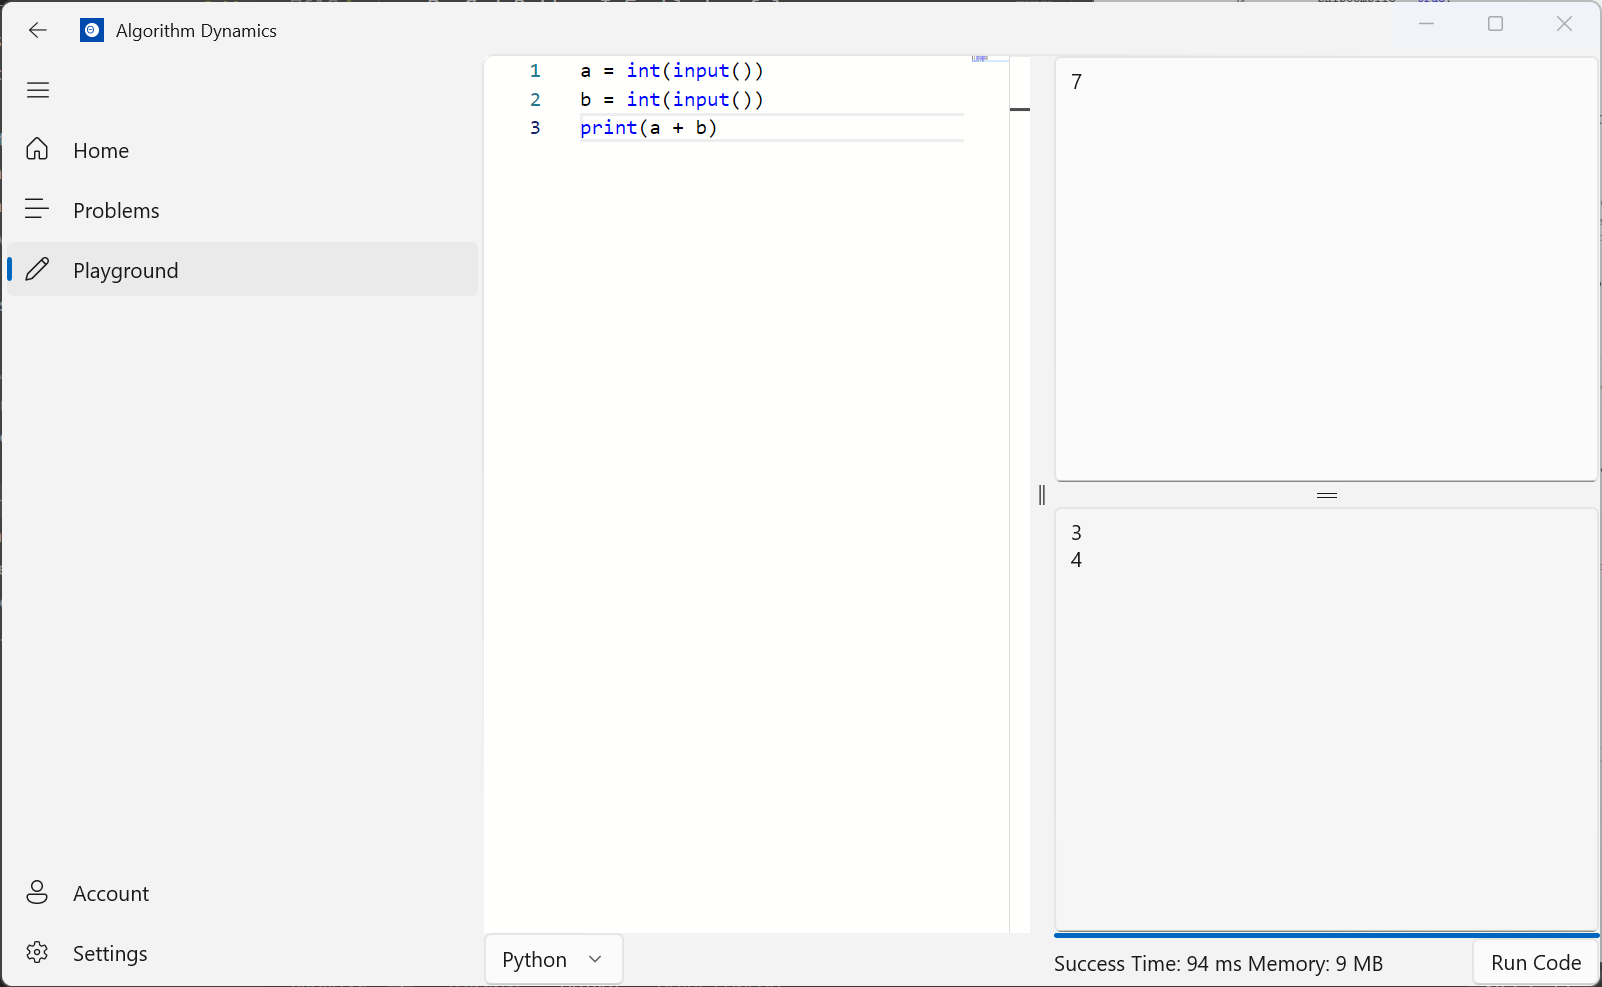
\includegraphics[width=\textwidth, height=\textheight, keepaspectratio]{PlaygroundPage-RunCode}

The RunCode function in the CodingPage is similar. Please refer to the source code for the detailed implementation.

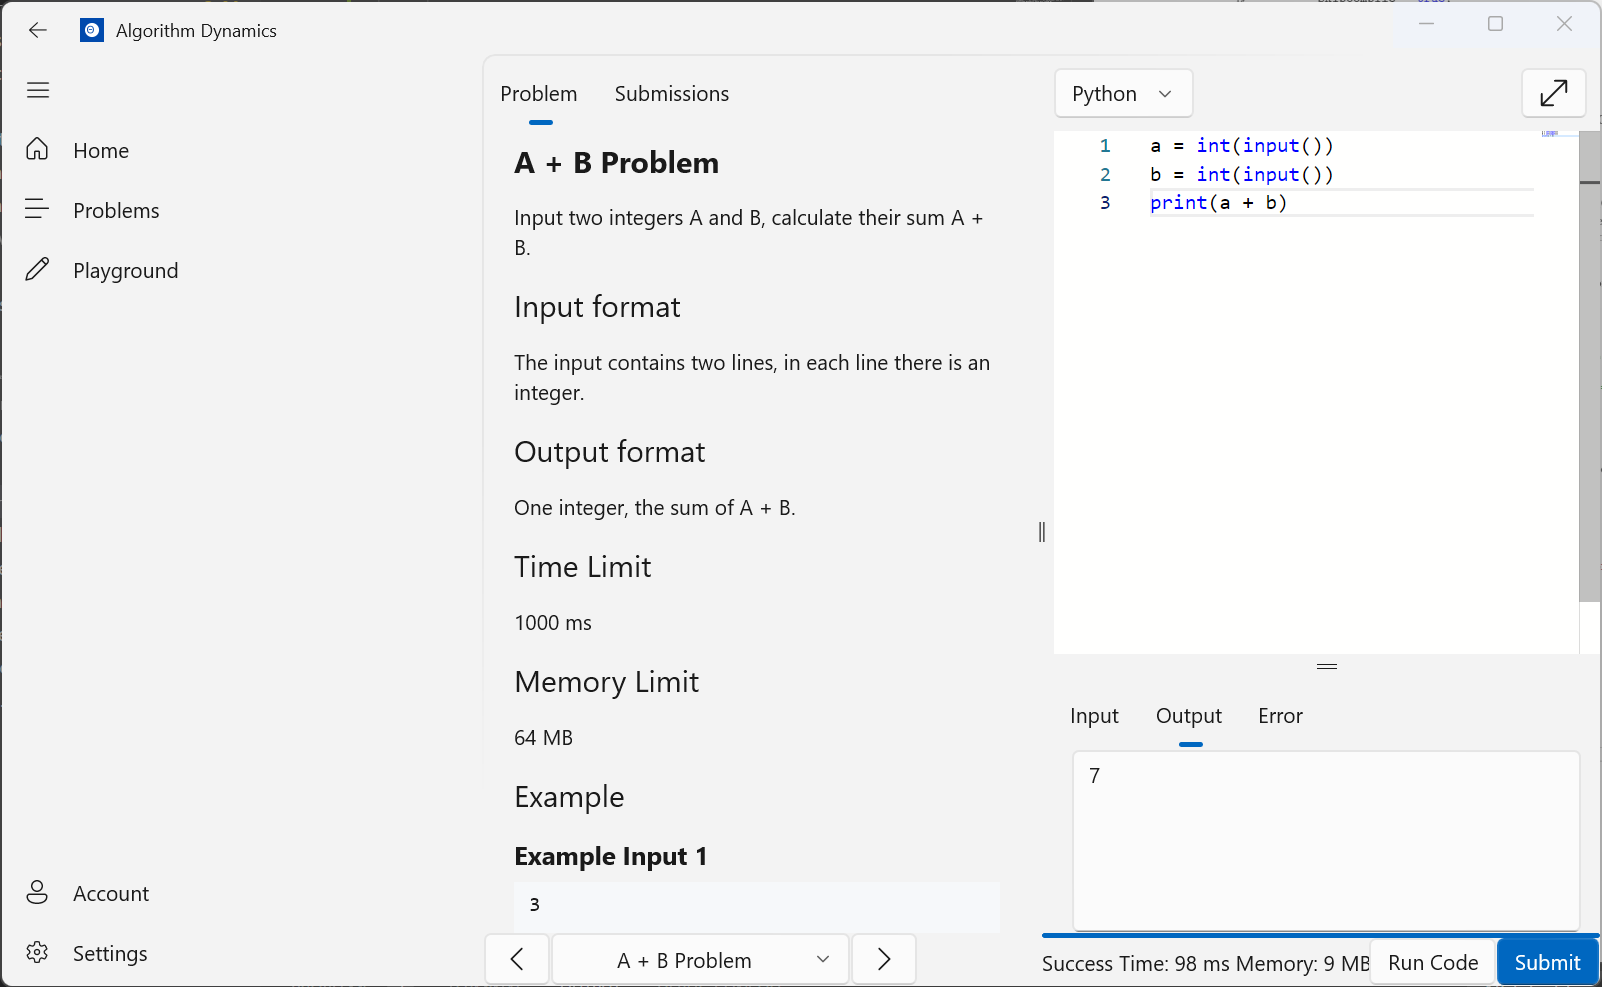
\includegraphics[width=\textwidth, height=\textheight, keepaspectratio]{CodingPage-RunCode}

The submission button creates a formal submission and commits the result to the database.

\begin{minted}{csharp}
/// <summary>
/// Submit the user's code for formal judging
/// </summary>
/// <param name="sender"></param>
/// <param name="e"></param>
private async void SubmitCodeButton_Click(object sender, RoutedEventArgs e)
{
    // Create submission
    Submission submission = Submission.Create(CodeEditor.Code, (Language)LanguageComboBox.SelectedItem, App.CurrentUser, _currentProblem);
    
    // Prepare progerss bar and button
    var progress = new Progress<int>(percent => { RunCodeProgressBar.Value = percent; });
    RunCodeButton.IsEnabled = false;
    SubmitCodeButton.IsEnabled = false;

    // Judge problem
    SubmissionResult result = await Judger.JudgeProblem(submission, progress);

    // Restore button
    RunCodeButton.IsEnabled = true;
    SubmitCodeButton.IsEnabled = true;

    // Display the result
    StatusTextBlock.Text = $"{result.Result} Time: {result.CPUTime} ms Memory: {result.MemoryUsage / 1024 / 1024} MB";
    ErrorTextBox.Text = result.StandardError;
    
    // Navigate to stderr
    if (!string.IsNullOrWhiteSpace(result.StandardError))
    {
        IOPivot.SelectedIndex = 2;
    }
    OnPropertyChanged(nameof(Submissions));
    OnPropertyChanged(nameof(ReverseSubmissions));
}
\end{minted}

The submission is graded correctly.

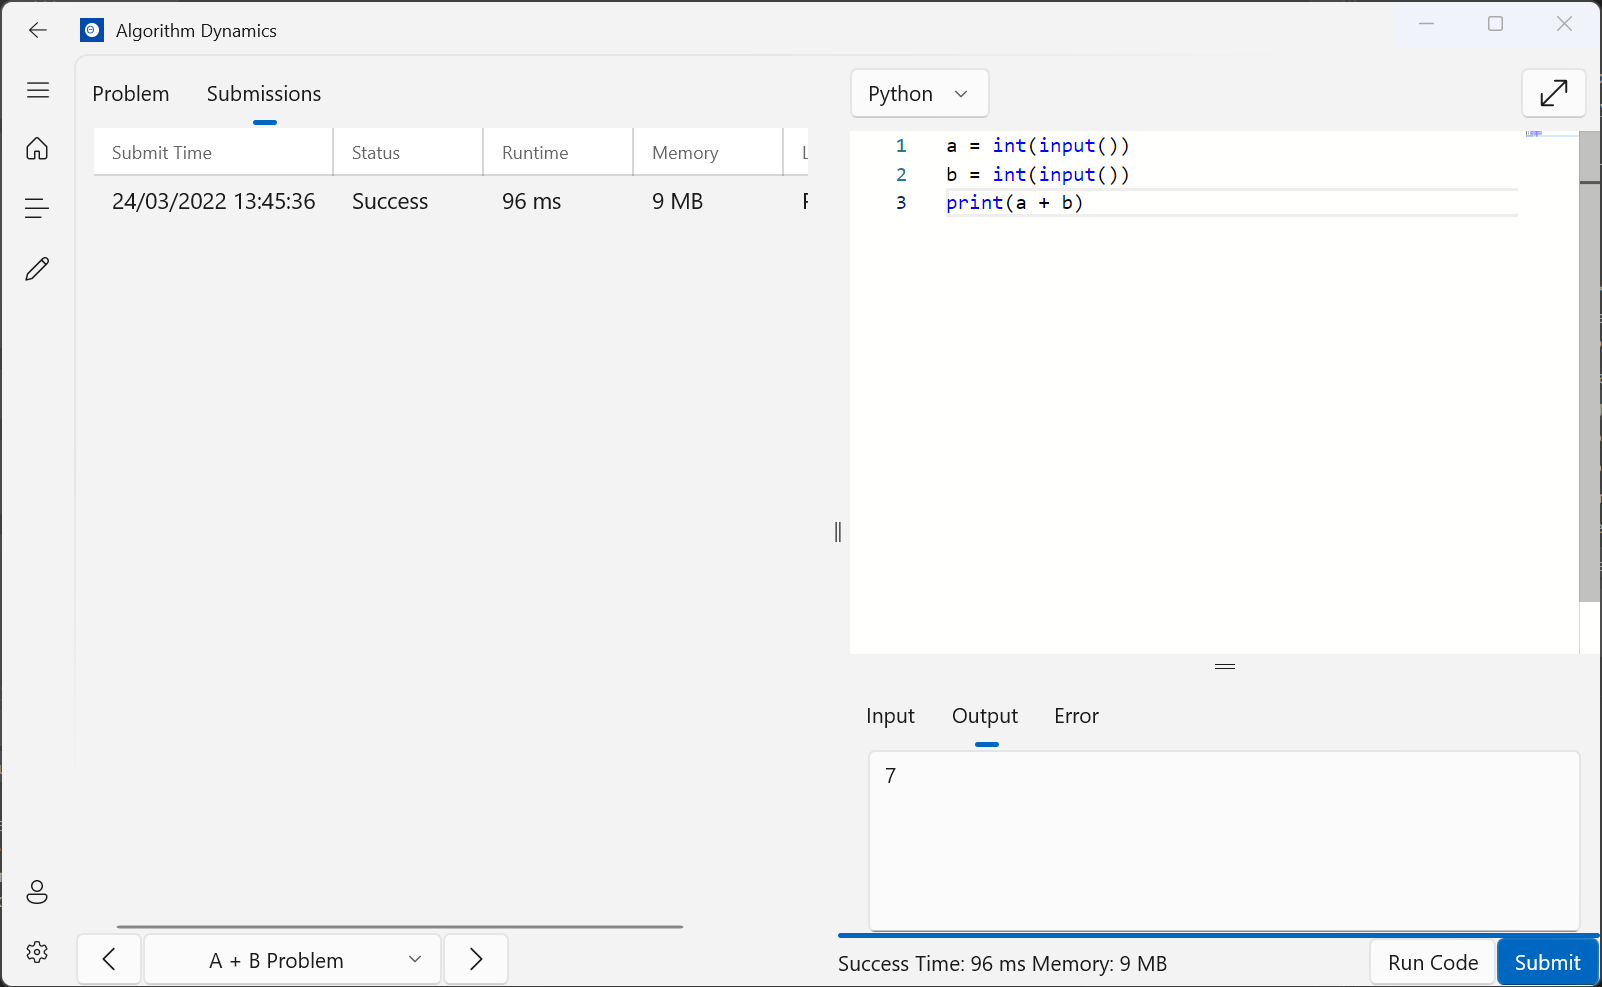
\includegraphics[width=\textwidth, height=\textheight, keepaspectratio]{CodingPage-Submit}

The Judger is implemented and fully tested, I will hand this to the stakeholders for their feedback.

\subsection{Stakeholder feedback}

PCloud reported that the Judger will panic when the language config is not correct. This is a very serious issue, the Judger should not crash under any circumstances. I can reproduce it in my environment.

\begin{minted}{text}
Message:
Test method Algorithm_Dynamics.Test.TestJudger.TestRunCodeCpp threw exception:
System.ComponentModel.Win32Exception: An error occurred trying to start process 'g--' with working directory '.'. The system cannot find the file specified.

Stack Trace:
Process.StartWithCreateProcess(ProcessStartInfo startInfo)
Process.Start()
Judger.Compile(Language language) line 66
Judger.RunCode(String UserCode, String Input, Language language, Int32 TimeLimit, Int64 MemoryLimit, IProgress`1 Progress) line 218
TestJudger.TestRunCodeCpp() line 34
ThreadOperations.ExecuteWithAbortSafety(Action action)
\end{minted}

If the compiler does not exist on the path, the Judger will panic directly. This should be handled more gracefully and a proper error should be reported. I can add a check for the compiler's existence before running.

I set up a function \code{GetFullPath} to search the local folder and environment variable path for a given file. It returns null if the file is not found.

\begin{minted}{csharp}
/// <summary>
/// Search local and environment variable to get the full path of a file.
/// Return <see cref="null"/> if the file does not exist.
/// </summary>
/// <param name="fileName"></param>
/// <returns></returns>
private static string GetFullPath(string fileName)
{
    // Check whether the file exists in the local folder
    if (File.Exists(fileName))
        return Path.GetFullPath(fileName);

    // Check the environment variable
    var values = Environment.GetEnvironmentVariable("PATH");
    foreach (var path in values.Split(Path.PathSeparator))
    {
        var fullPath = Path.Combine(path, fileName);
        if (File.Exists(fullPath))
            return fullPath;
    }
    return null;
}
\end{minted}

Then I set up another function \code{ExistsOnPath} which returns a boolean value to check whether the compiler exists.

\begin{minted}{csharp}
/// <summary>
/// Check whether a file exist in the local folder or in the environment variable path.
/// </summary>
/// <param name="fileName"></param>
/// <returns></returns>
private static bool ExistsOnPath(string fileName)
{
    return GetFullPath(fileName) != null;
}
\end{minted}

Both methods are set to private as they are only intended to be used inside the \code{Judger} class.

Now, I can check whether the compile exists before compiling. A system error will be reported if it encounters an error.

\begin{minted}{csharp}
// Compile if needed
if (language.NeedCompile)
{
    // Check if the compiler exists before compiling
    if (!ExistsOnPath(language.CompileCommand.Replace("{SourceCodeFilePath}", sourceFilePath).Replace("{ExecutableFilePath}", _ExecutableFilePath)))
    {
        Progress.Report(100);
        result.StandardError = $"The CompileCommand {language.CompileCommand} cannot be found.\nPlease check the programming language configuration.";
        result.ResultCode = ResultCode.SYSTEM_ERROR;
        return result;
    }

    // Compile and report any error
    if (await Compile(language) != 0)
    {
        Progress.Report(100);
        result.StandardOutput = _CompilationOutput;
        result.StandardError = FilterErrorMessage(_CompilationError);
        result.ResultCode = ResultCode.COMPILE_ERROR;
        return result;
    }
}
\end{minted}

I also add a unit test to verify this error is fixed. It sets up an invalid compiler command and checks whether the Judger will report the correct error message.

\begin{minted}{csharp}
[TestMethod, TestCategory("TestSystemError")]
public async Task TestCompileSystemError()
{
    // Set up a non-exsiting compiler g--
    RunCodeResult result = await Judger.RunCode(
        helloWorldCpp,
        "",
        new("C++", "cpp", ".cpp", true, "g--", "-x c++ {SourceCodeFilePath} -o {ExecutableFilePath}", "{ExecutableFilePath}", ""),
        1 * S,
        64 * MB,
        new Progress<int>()
    );
    // Check the result code and error message
    Assert.AreEqual(result.ResultCode, ResultCode.SYSTEM_ERROR);
    Assert.AreEqual(result.StandardError, $"The CompileCommand g-- cannot be found.\nPlease check the programming language configuration.");
}
\end{minted}

I noticed another issue, the Judger can encounter the same issue when executing as well. For interpreting language like Python, the interpreter is called during execution, so its path must be checked before executing as well. Since I have written the function for \code{ExistsOnPath} it is easy to set up another check before executing.

\begin{minted}{csharp}
// Check run command before running
if (!ExistsOnPath(language.RunCommand.Replace("{SourceCodeFilePath}", sourceFilePath).Replace("{ExecutableFilePath}", _ExecutableFilePath)))
{
    Progress.Report(100);
    result.StandardError = $"The RunCommand {language.RunCommand} cannot be found.\nPlease check the programming language configuration.";
    result.ResultCode = ResultCode.SYSTEM_ERROR;
    return result;
}
\end{minted}

I also add the unit test for the execution case.

\begin{minted}{csharp}
[TestMethod, TestCategory("TestSystemError")]
public async Task TestExecuteSystemError()
{
    // Set up a non-exsiting interpreter p
    RunCodeResult result = await Judger.RunCode(
        helloWorldCpp,
        "",
        new("Python", "python", ".py", "p", "{SourceCodeFilePath}"),
        1 * S,
        64 * MB,
        new Progress<int>()
    );
    // Check the result code and error message
    Assert.AreEqual(result.ResultCode, ResultCode.SYSTEM_ERROR);
    Assert.AreEqual(result.StandardError, $"The RunCommand p cannot be found.\nPlease check the programming language configuration.");
}
\end{minted}

Both tests passed successfully.

\begin{minted}{text}
> dotnet test --filter TestCategory=TestSystemError
  Determining projects to restore...
  All projects are up-to-date for restore.
  Algorithm Dynamics.Core -> C:\Algorithm-Dynamics\src\Algorithm Dynamics.Core\bin\Debug\net6.0\Algorithm Dynamics.Core.dll
  Algorithm Dynamics.Test -> C:\Algorithm-Dynamics\src\Algorithm Dynamics.Test\bin\Debug\net6.0\Algorithm Dynamics.Test.dll
Test run for C:\Algorithm-Dynamics\src\Algorithm Dynamics.Test\bin\Debug\net6.0\Algorithm Dynamics.Test.dll (.NETCoreApp,Version=v6.0)
Microsoft (R) Test Execution Command Line Tool Version 17.0.0
Copyright (c) Microsoft Corporation.  All rights reserved.

Starting test execution, please wait...
A total of 1 test files matched the specified pattern.

Passed!  - Failed:     0, Passed:     2, Skipped:     0, Total:     2, Duration: 49 ms - Algorithm Dynamics.Test.dll (net6.0)
\end{minted}

I then test it in the integration environment, the error message is displayed correctly and so is the error code.

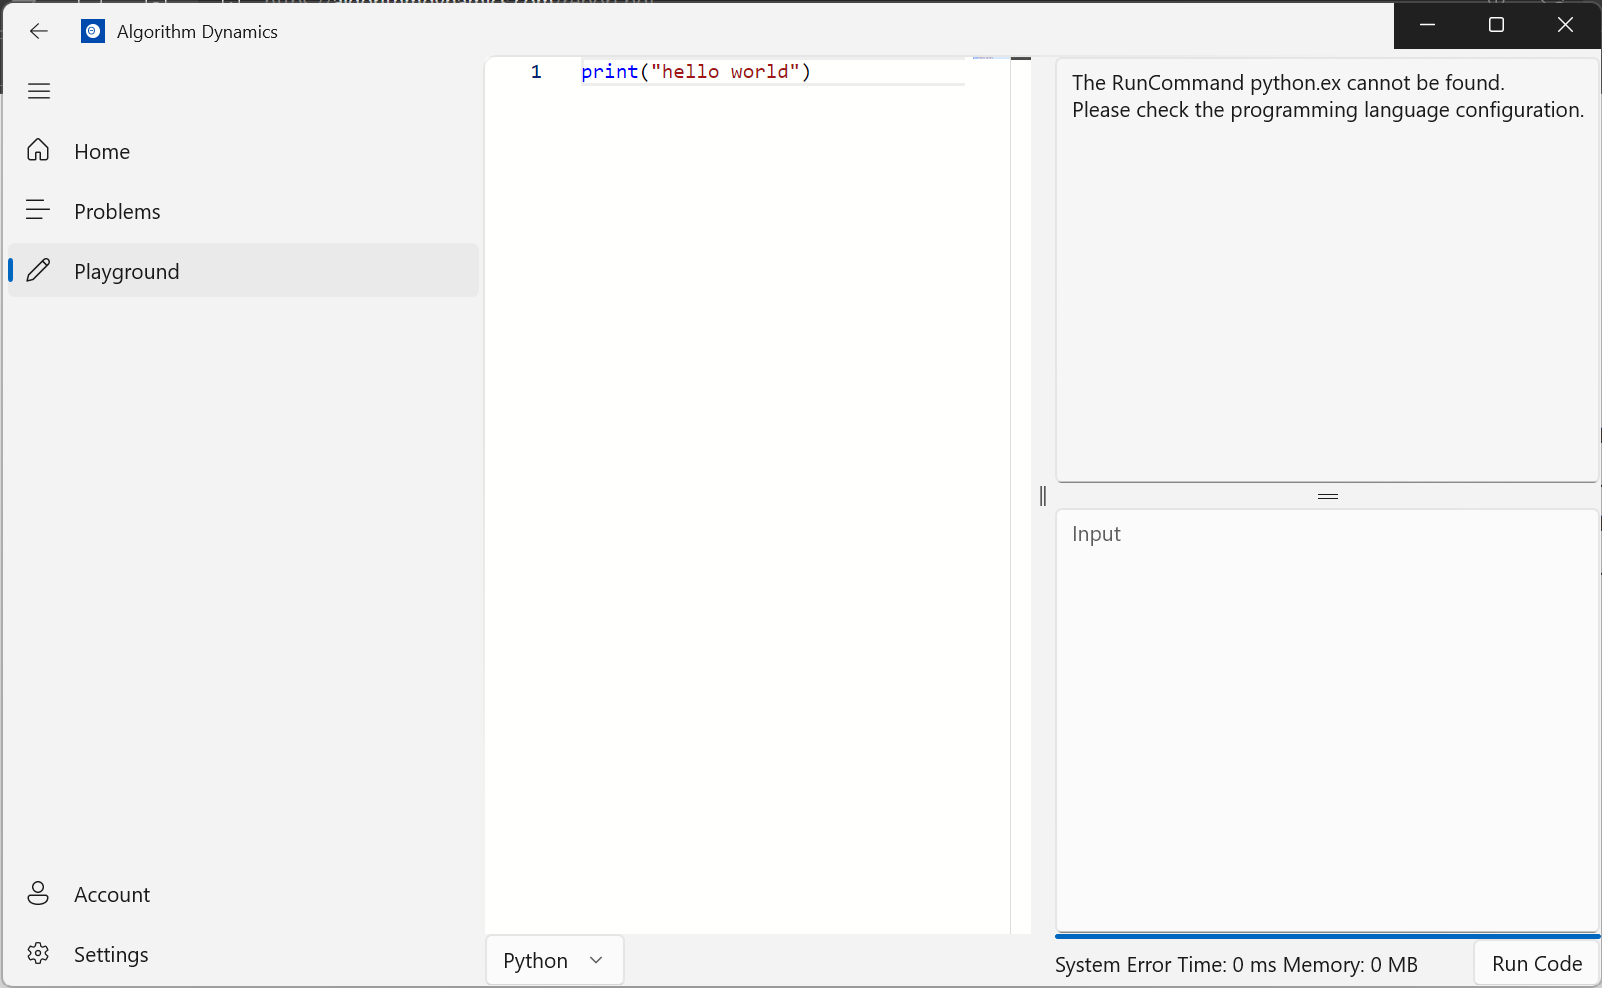
\includegraphics[width=\textwidth, height=\textheight, keepaspectratio]{SystemErrorReport}

I show this result back to the stakeholder, and he is happy with how I handle this error.

Timofei reports that the judging speed is very slow with multiple test cases on compiling language. After some investigation, I found that the reason is that the same source code gets compiled whenever a test case is evaluated. I can optimize the \code{RunCode} function to skip compile after the first test case.

\begin{minted}{csharp}
public async static Task<RunCodeResult> RunCode(string UserCode, string Input, Language language, int TimeLimit, long MemoryLimit, IProgress<int> Progress = null, bool skipCompile = false)
{
    // ...

    // Compile if needed
    if (language.NeedCompile && (!skipCompile))
    {
        // ...
    }

    // ...
}
\end{minted}


\begin{minted}{csharp}
public async static Task<SubmissionResult> JudgeProblem(Submission Submission, IProgress<int> Progress)
{
    // ...

    bool skipCompile = false;
    while (JudgeQueue.Count > 0)
    {
        TestCaseResult result = await JudgeTestCase(
            Submission.Code,
            JudgeQueue.Dequeue(),
            Submission.Language,
            Submission.Problem.TimeLimit,
            Submission.Problem.MemoryLimit,
            skipCompile);

        // ...

        // Skip compile
        skipCompile = true;
    }

    // ...
}
\end{minted}

Now each code submission will only get compiled once, and therefore the total judging time is shortened significantly. Timofei is satisfied with this result.

\end{document}